\section{System Design}

In order to develop the system, only front-end technologies will be user. Additional to HTML5, CSS3 and vanilla JS, Vue.js framework is planned to use. Vue framework will make easier for development also helps get rid of boiler-code.

The reflection of main page can be seen in figure 1 (the figures contains links to higher resolution images). The main page contains several links. First link directs to Mark-Down to HTML converter. Second link directs to Presentation Generator in order to generate presentations using already generated HTML pages.

In the last part of the main page, already generated presentations are displayed. Each newly generated presentation will be added to here.

\begin{figure}[h]
    \href{https://raw.githubusercontent.com/krmacit/SWE599-Project-Report-2021S-Macit-KerimCan/master/Mockups/MainPage.png}{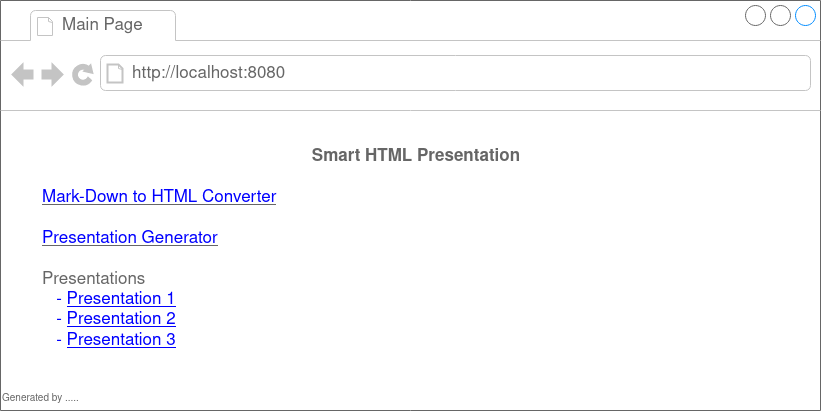
\includegraphics[scale=0.31]{Mockups/MainPage.png}}
    \caption{Main Page}
\end{figure}


\subsection{Mark-Down to HTML Generator}

Mark-Down to HTML part consist of 3 parts. In the top bar, new generated page name and location is to be determined. Also the container consist of save button to save generated HTML page. The main part is consist of 2 pages. In the left part, it is expected to input MD from user and accordingly generated image will be shown in the left frame. The mock-up can be seen in figure 2.

\begin{figure}[h]
    \href{https://raw.githubusercontent.com/krmacit/SWE599-Project-Report-2021S-Macit-KerimCan/master/Mockups/MarkdownToHTML.png}{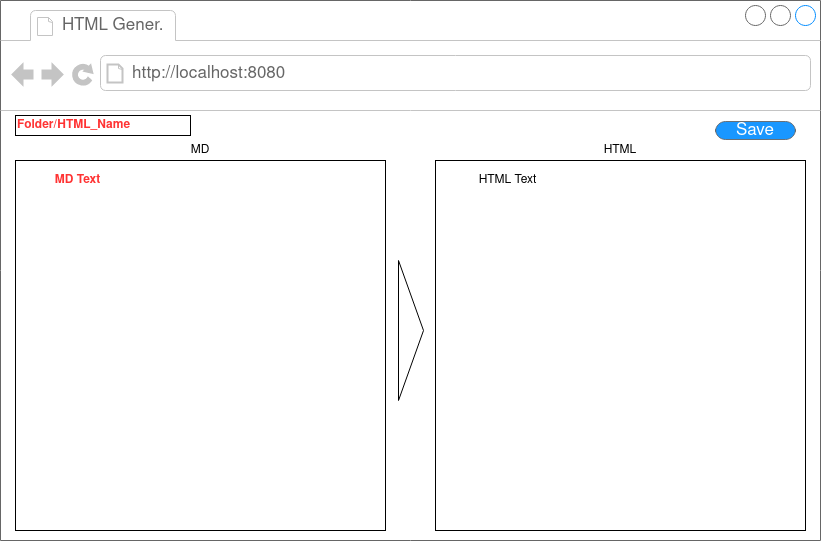
\includegraphics[scale=0.3]{Mockups/MarkdownToHTML.png}}
    \caption{Slide Page}
\end{figure}

\subsection{Presentation Generator}

The presentation generator has also similar top bar, generated presentation name and save button. In the main part of the page, all generated pages is shown with grouping according to containing folder. Each presentation has also input form which shows the slide order.

The system will generate the presentation with inputted order. The system does not allow user to give same order number to more than one slide.

\begin{figure}[h]
    \href{https://raw.githubusercontent.com/krmacit/SWE599-Project-Report-2021S-Macit-KerimCan/master/Mockups/PresentationGenerator.png}{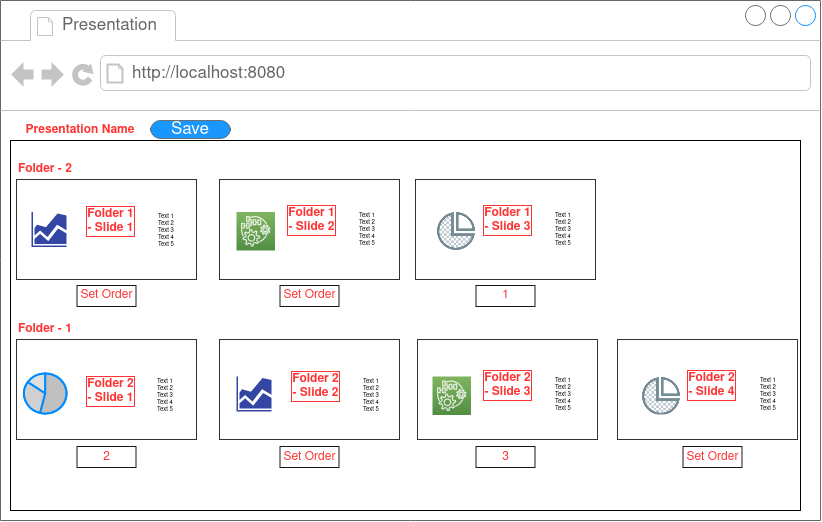
\includegraphics[scale=0.3]{Mockups/PresentationGenerator.png}}
    \caption{Presentation Generator Page}
\end{figure}

\subsection{Presentation Navigation System}

Last part of the system is navigation system. The system shows navigation tools, forward and backward button. The buttons in the below has also table of content system. The page mock-up can be seen in figure 2. These buttons are visible only when the mouse button hovers towards it, otherwise it will be invisible.

\begin{figure}[h]
    \href{https://raw.githubusercontent.com/krmacit/SWE599-Project-Report-2021S-Macit-KerimCan/master/Mockups/NavigationSystem_1.png}{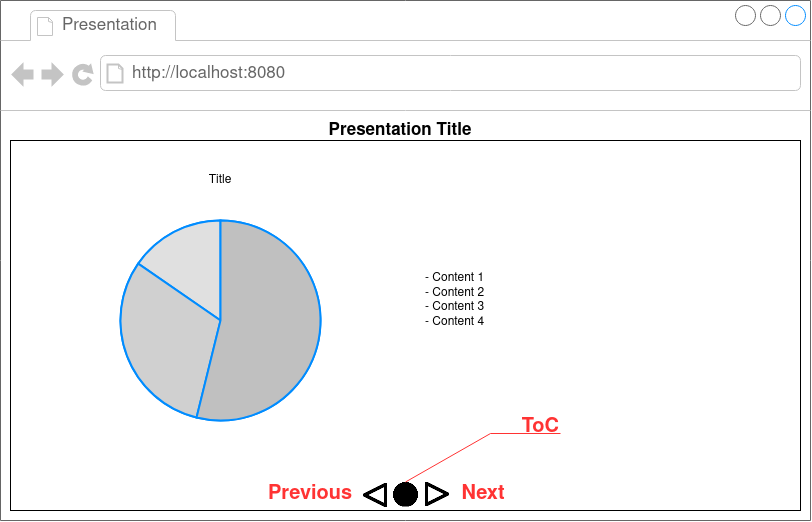
\includegraphics[scale=0.32]{Mockups/NavigationSystem_1.png}}
    \caption{Presentation Navigation Page}
\end{figure}

The table of content will be opened over current presentation page. It shows all the pages the presentation consists. Selecting any page will direct to that page. 

\begin{figure}[h]
\href{https://raw.githubusercontent.com/krmacit/SWE599-Project-Report-2021S-Macit-KerimCan/master/Mockups/NavigationSystem_2.png}{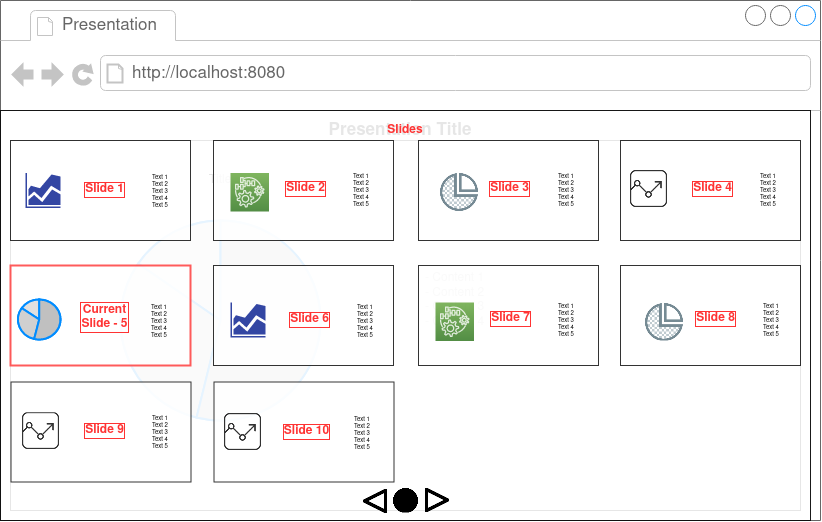
\includegraphics[scale=0.315]{Mockups/NavigationSystem_2.png}}
    \caption{Table of Content Page}
\end{figure}